% Compile with: pdflatex presentation.tex (twice)
% Requires the `metropolis` theme (TeX Live: package `beamertheme-metropolis`).
% If unavailable, change \usetheme{metropolis} to \usetheme{default} below.
% NOTE: not compiled locally (no pdflatex/xelatex in this environment) -- verify
% with a real LaTeX pass before presenting. Figures copied in from
% docs/figures/ and experiments/latest/*/plot.png (real run outputs, not mockups).

\documentclass[10pt,aspectratio=169]{beamer}

\usetheme{metropolis}
\metroset{progressbar=frametitle, sectionpage=progressbar, numbering=fraction}

\usepackage{booktabs}
\usepackage{graphicx}
\usepackage{amsmath}
\usepackage{xcolor}

\definecolor{accent}{HTML}{2980b9}
\definecolor{good}{HTML}{27ae60}
\definecolor{bad}{HTML}{c0392b}
\setbeamercolor{progress bar}{fg=accent}
\setbeamercolor{title separator}{fg=accent}

\setbeamerfont{title}{size=\Large, series=\bfseries}
\setbeamerfont{frametitle}{size=\normalsize, series=\bfseries}
\setbeamerfont{caption}{size=\scriptsize}

\newcommand{\tk}[1]{{\scriptsize \textcolor{accent}{$\blacktriangleright$}\ #1}}

\title{7B-Scale Validation}
\subtitle{Beating DISP-LLM, training discipline at scale, and what downstream eval actually shows}
\author{Keshava Pampatti}
\date{\today}

\graphicspath{{./}}

\begin{document}

\maketitle

% ============================================================
\begin{frame}{What this talk covers}
  \begin{itemize}
    \item Everything here is the \textbf{same pruner} (row-encoder + BiLSTM, $\approx$2M params) that ran on GPT-2/OPT-125M --- no architecture change, only the weight-extraction plumbing differs per model.
    \item Three real 7B-scale sweeps: \textbf{Llama-2-7B / WikiText-2}, \textbf{Mistral-7B / C4}, \textbf{Mistral-7B / WikiText-2}. Plus one first look at a downstream-task objective (\textbf{CNN/DailyMail}).
  \end{itemize}
  \vspace{0.6em}
  \begin{block}{Headline}
    On the one directly matched comparison available in the literature (Llama-2-7B, WikiText-2, no-weight-update), we \textbf{beat DISP-LLM's own published numbers at every converged operating point}. Downstream zero-shot accuracy tells a more complicated story --- covered honestly, not smoothed over.
  \end{block}
\end{frame}

% ============================================================
\section{Training regime \& the convergence check}
% ============================================================

\begin{frame}{The objective, unchanged from GPT-2/OPT-125M}
  Frozen base model, only the pruner $\phi$ trains:
  \[
    \mathcal{L} = (\text{CE}_{\text{pruned}} - \text{CE}_{\text{orig}}) + \lambda \cdot \overline{\text{gate}}
  \]
  \begin{itemize}
    \item Forward pass runs \textbf{twice} per step --- once ungated (CE$_{\text{orig}}$, no\_grad), once gated (CE$_{\text{pruned}}$, gradients flow only into $\phi$).
    \item $\lambda$ is the sole sparsity/accuracy knob, swept per model.
    \item Everything at 7B scale trains this way with \emph{no per-model tuning} beyond the weight-extraction plumbing.
  \end{itemize}
  \vspace{0.5em}
  \tk{What's new at this scale isn't the objective --- it's needing to know \emph{when to stop}, cheaply, without a hand-picked step count. That's the convergence check.}
\end{frame}

\begin{frame}{Convergence check: block-mean flatness, not a fixed step count}
  \begin{columns}[T,onlytextwidth]
    \column{0.55\textwidth}
      Every \texttt{check\_every} steps, compare the last \texttt{window} block-means of each layer's keep-rate history against the most recent one:
      \[
        \bar{k}_\ell(cp) = \frac{1}{\text{check\_every}} \sum_{s=cp-\text{check\_every}}^{cp} k_\ell(s)
      \]
      \[
        \text{tol} = \max(\text{rel\_tol}\cdot|\bar{k}_\ell^{\text{ref}}|,\ \text{abs\_tol})
      \]
      \textbf{Raw signal} fires only if \emph{every layer} is within tol of the reference, for \emph{every} checkpoint in the window, after a \texttt{burn\_in} floor.
    \column{0.45\textwidth}
      \begin{block}{Why per-layer, not global}
        A global average can look flat while individual layers are still trading pruned neurons back and forth --- the check has to fail if \emph{any} layer is still moving.
      \end{block}
  \end{columns}
\end{frame}

\begin{frame}{B9: don't trust the first flat window}
  \begin{columns}[T,onlytextwidth]
    \column{0.55\textwidth}
      A raw signal can be a plateau, or just noise sitting still under a constant LR. So it doesn't confirm convergence --- it triggers a \textbf{cosine LR decay} first:
      \[
        \text{lr}(s) = \text{lr}_{\min} + \tfrac12(\text{lr}_0-\text{lr}_{\min})\Big(1+\cos\tfrac{\pi s}{W}\Big)
      \]
      After $W$ steps at $\text{lr}_{\min}$, \textbf{re-check}. Passes $\Rightarrow$ confirmed converged. Fails $\Rightarrow$ hold at $\text{lr}_{\min}$, keep training (\texttt{post\_decay}) --- the original signal was noise the higher LR was masking.
    \column{0.45\textwidth}
      \begin{center}\small
        \texttt{pre\_decay} $\to$ \texttt{decaying} $\to$ \{\texttt{CONFIRMED}, \texttt{post\_decay}\}
      \end{center}
      \vspace{0.4em}
      \tk{This three-state machine is what lets every sweep in this talk report ``converged'' as a checked fact, not an assumption.}
  \end{columns}
\end{frame}

% ============================================================
\section{Mistral-7B: does the method just work elsewhere?}
% ============================================================

\begin{frame}{Mistral-7B / C4 --- same shape, one real wrinkle}
  \begin{columns}[T,onlytextwidth]
    \column{0.5\textwidth}
      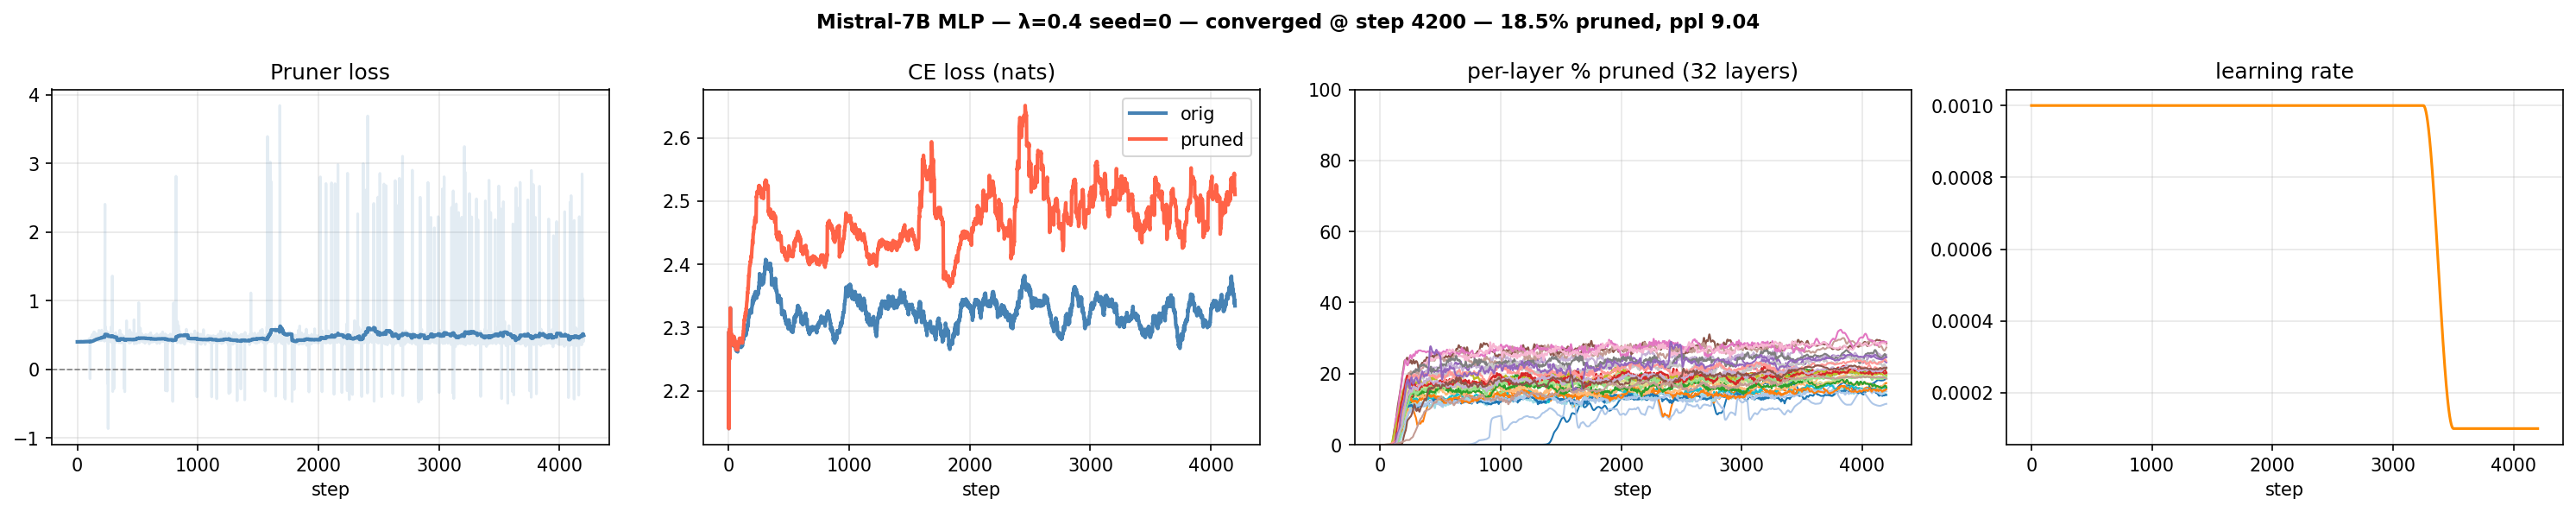
\includegraphics[width=\linewidth]{mistral_c4_lambda04.png}
    \column{0.5\textwidth}
      Same free-region-then-monotonic-cost shape seen at every smaller scale.
      \vspace{0.4em}

      \textbf{One non-monotonicity}: $\lambda{=}0.3\to0.4$ prunes \emph{more} for \emph{less} cost --- not a real reversal. $\lambda{=}0.4$'s convergence trigger simply fired much later (4200 vs.\ 1150 steps), so it completed far more of its trajectory before the check stopped it.
      \vspace{0.4em}
      \tk{Same mechanism as the capacity-axis finding from GPT-2/OPT-125M (F3) --- window validity depends on how much of the run has actually finished, now showing up along $\lambda$ instead of capacity.}
  \end{columns}
\end{frame}

\begin{frame}{Mistral-7B / WikiText-2 --- a smaller curve, and why}
  \begin{itemize}
    \item Dense baseline ppl: \textbf{4.740} (WikiText-2) vs.\ \textbf{8.325} (C4) --- Mistral is already well-calibrated to clean Wikipedia-style text.
    \item Consequence: much less redundancy to find on WikiText-2 specifically --- the whole sparsity/cost curve sits closer to the axis than C4's.
  \end{itemize}
  \vspace{0.5em}
  \tk{Exactly the concern flagged \emph{before} running it: a model already well-matched to a domain has less slack for a pruner to discover in the first place.}
\end{frame}

% ============================================================
\section{Beating DISP-LLM}
% ============================================================

\begin{frame}{Setup: the one directly matched comparison available}
  \begin{itemize}
    \item DISP-LLM (Gao 2024) reports LLaMA-2-7B, WikiText-2, \textbf{no weight update} --- same model, same dataset, same ``frozen weights'' framing this project already uses.
    \item Our 9-$\lambda$ convergence-based sweep, converted to \textbf{total-param-pruned \%} via Llama-2-7B's 64.24\% MLP parameter share, plotted directly against DISP-LLM's own published Table 1 numbers (linearly interpolated between their 5 reported points).
  \end{itemize}
  \vspace{0.4em}
  \tk{No re-running DISP-LLM's code, no proxy dataset --- their own numbers, our own numbers, same axis.}
\end{frame}

\begin{frame}{8 of 8 converged points beat the interpolated DISP-LLM curve}
  \begin{columns}[T,onlytextwidth]
    \column{0.52\textwidth}
      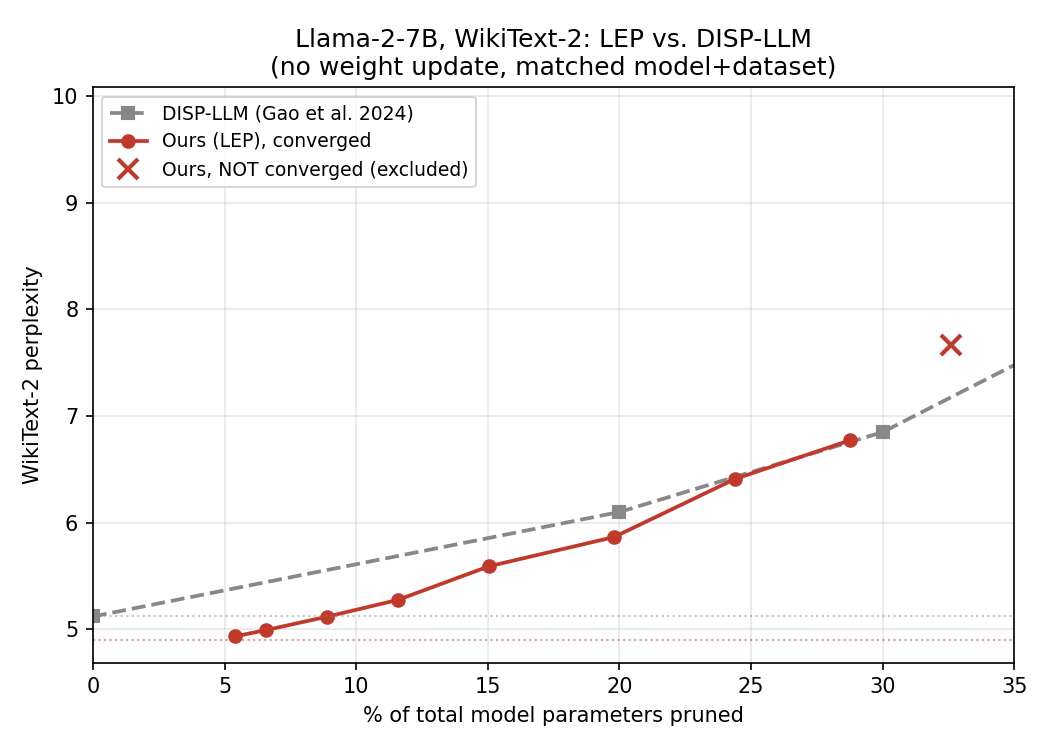
\includegraphics[width=\linewidth]{disp_llm.png}
    \column{0.48\textwidth}
      Dense ppl: ours \textbf{4.903} vs.\ DISP-LLM's \textbf{5.12}.
      \begin{itemize}
        \item $-0.45$ ppl at the low end (5.4--6.6\% total pruned)
        \item narrowing to a near-tie ($+0.016$ ppl) at 28.77\%
      \end{itemize}
      \vspace{0.4em}
      \tk{Every converged point beats it. The margin shrinks as sparsity grows, but never flips negative for any point that actually converged.}
  \end{columns}
\end{frame}

\begin{frame}{The 9th point --- diagnosed, not hidden}
  \begin{columns}[T,onlytextwidth]
    \column{0.5\textwidth}
      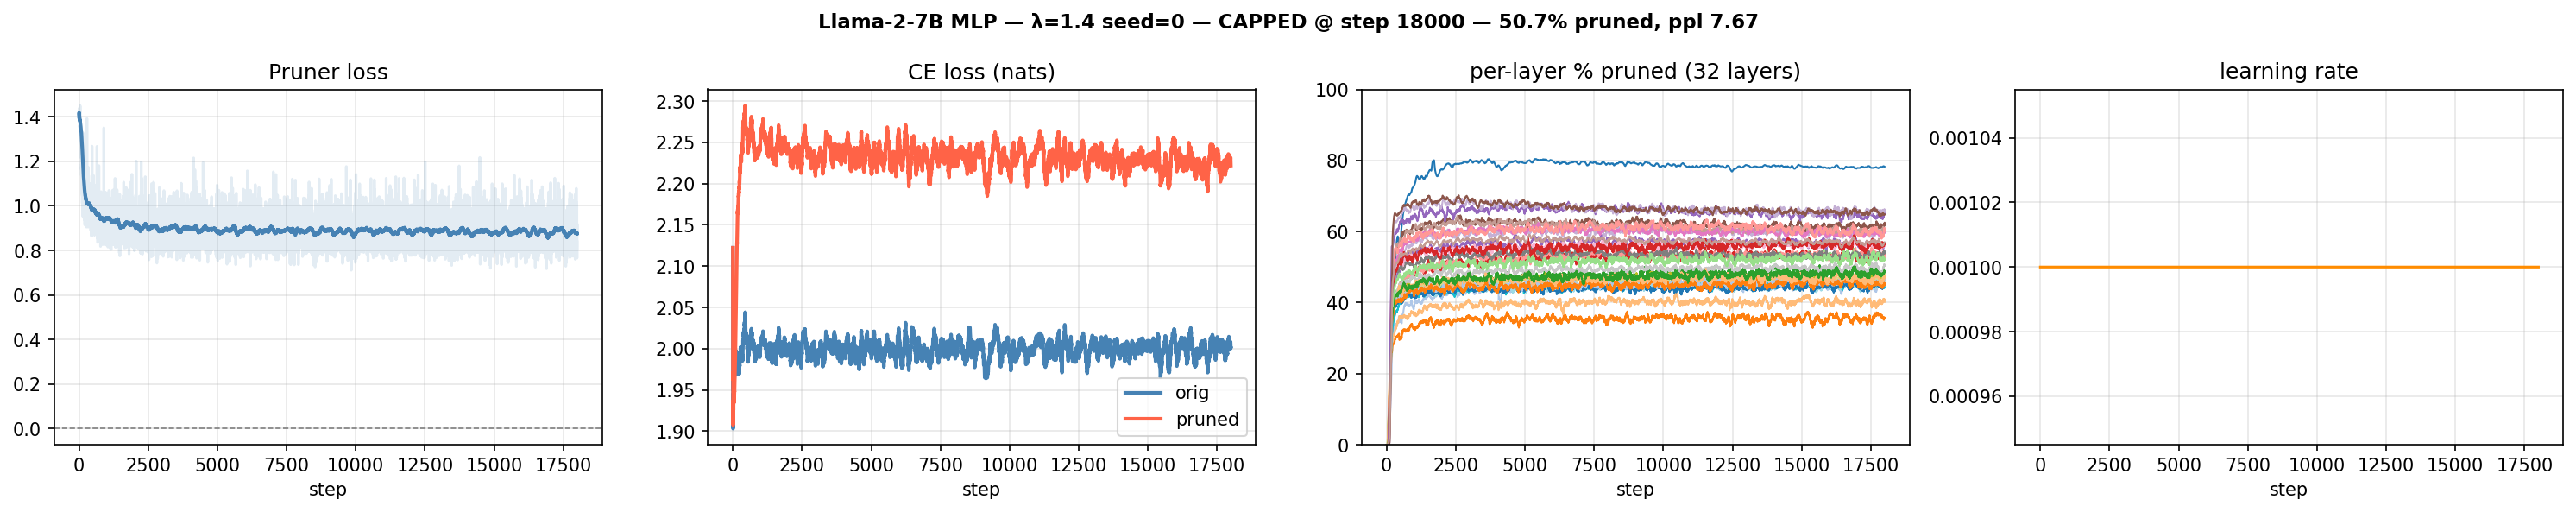
\includegraphics[width=\linewidth]{lambda14_nonconverged.png}
    \column{0.5\textwidth}
      $\lambda{=}1.4$ (32.6\% total pruned) loses to DISP-LLM by $+0.494$ ppl --- but it \textbf{never converged}: \texttt{pre\_decay} for the entire 18{,}000-step cap.
      \vspace{0.4em}

      \texttt{pct\_pruned} still swings an 8.2pp band in the \emph{final} 20 checkpoints; individual layers still move $\sim$30--48pp step-to-step at step 18{,}000. A sustained oscillation, not a slow approach to a plateau.
      \vspace{0.3em}
      \tk{Excluded from the headline claim on that basis --- not a cherry-picked drop.}
  \end{columns}
\end{frame}

\begin{frame}{Why it oscillates, and why ``bigger pruner'' isn't the fix}
  \begin{itemize}
    \item At $\lambda{=}1.4$ the sparsity term ($\approx 0.66$--$0.8$) is now comparable in size to the CE-cost term ($\approx 0.37$--$0.46$) --- and LR is held at a constant $10^{-3}$ regardless of $\lambda$, since B9's decay never gets to intervene without a raw signal firing first.
    \item Directly tested ``increase pruner capacity'' against this project's own prior evidence (an 8-point matched grid at half/base/2.26$\times$ capacity, GPT-2+OPT-125M) --- \textbf{no monotonic capacity effect exists there} on \%pruned, ppl, or convergence speed.
  \end{itemize}
  \vspace{0.4em}
  \tk{Capacity controls the scorer's expressiveness, not the STE threshold's oscillation dynamics under a fixed-LR gradient. The indicated fix is LR/$\lambda$-coupling --- an optimization-dynamics diagnosis, not a capacity one. Not yet tested at 7B.}
\end{frame}

% ============================================================
\section{Downstream eval: the ppl win doesn't fully transfer}
% ============================================================

\begin{frame}{Same 8 checkpoints, lm-evaluation-harness, 0-shot}
  \begin{itemize}
    \item PIQA / HellaSwag / WinoGrande / ARC-e / ARC-c / BoolQ / OpenBookQA, run on all 8 converged checkpoints + dense.
    \item Restricted here to DISP-LLM's own 5-task subset (WinoGrande acc; HellaSwag/ARC-e/ARC-c/PIQA acc-norm) for a like-for-like comparison.
  \end{itemize}
  \vspace{0.4em}
  \tk{Closes a real gap this project's own venue-analysis flagged: perplexity alone isn't what the comparable literature reports as headline evidence.}
\end{frame}

\begin{frame}{Near-parity at light pruning, a growing deficit at heavy pruning}
  \begin{center}\scriptsize
  \begin{tabular}{@{}lrrr@{}}
    \toprule
    \% total params pruned & LEP avg acc & DISP-LLM (interp.) & LEP $-$ DISP-LLM \\
    \midrule
    0\% (dense) & 68.46 & 68.99 & $-0.53$ \\
    5.39\%      & 66.59 & 67.03 & $-0.44$ \\
    6.57\%      & 66.91 & 66.61 & $+0.30$ \\
    8.89\%      & 66.28 & 65.76 & $+0.52$ \\
    11.58\%     & 64.37 & 64.79 & $-0.42$ \\
    15.05\%     & 62.87 & 63.53 & $-0.66$ \\
    19.79\%     & 60.29 & 61.81 & $-1.52$ \\
    24.38\%     & 59.28 & 60.14 & $-0.86$ \\
    28.77\%     & 55.51 & 58.55 & $\mathbf{-3.04}$ \\
    \bottomrule
  \end{tabular}
  \end{center}
  \vspace{0.3em}
  \tk{Against DISP-LLM's own \emph{actually-measured} 30\% point (58.10, a slightly harder ratio than our 28.77\%) --- still behind by \textbf{2.59pp}, direct comparison, no interpolation.}
\end{frame}

\begin{frame}{The opposite shape from the perplexity result}
  \begin{columns}[T,onlytextwidth]
    \column{0.55\textwidth}
      \textbf{Perplexity (earlier)}: LEP starts ahead, margin \emph{narrows} toward high sparsity.
      \vspace{0.4em}

      \textbf{Downstream accuracy (here)}: LEP starts at parity, gap \emph{opens up} toward high sparsity.
    \column{0.45\textwidth}
      \begin{block}{Not yet explained}
        Candidate, untested: ppl is smooth and measured in-domain (WikiText-2, what the pruner was trained against); the downstream suite is discrete, out-of-domain, and may lean on specific circuits an in-domain-ppl-optimized mask doesn't protect.
      \end{block}
  \end{columns}
  \vspace{0.4em}
  \tk{Reported plainly because a reader who only sees the ppl table would draw a stronger conclusion than the data supports.}
\end{frame}

% ============================================================
\section{A first look: pruning for a downstream task}
% ============================================================

\begin{frame}{CNN/DailyMail --- one point, not a result yet}
  \begin{columns}[T,onlytextwidth]
    \column{0.5\textwidth}
      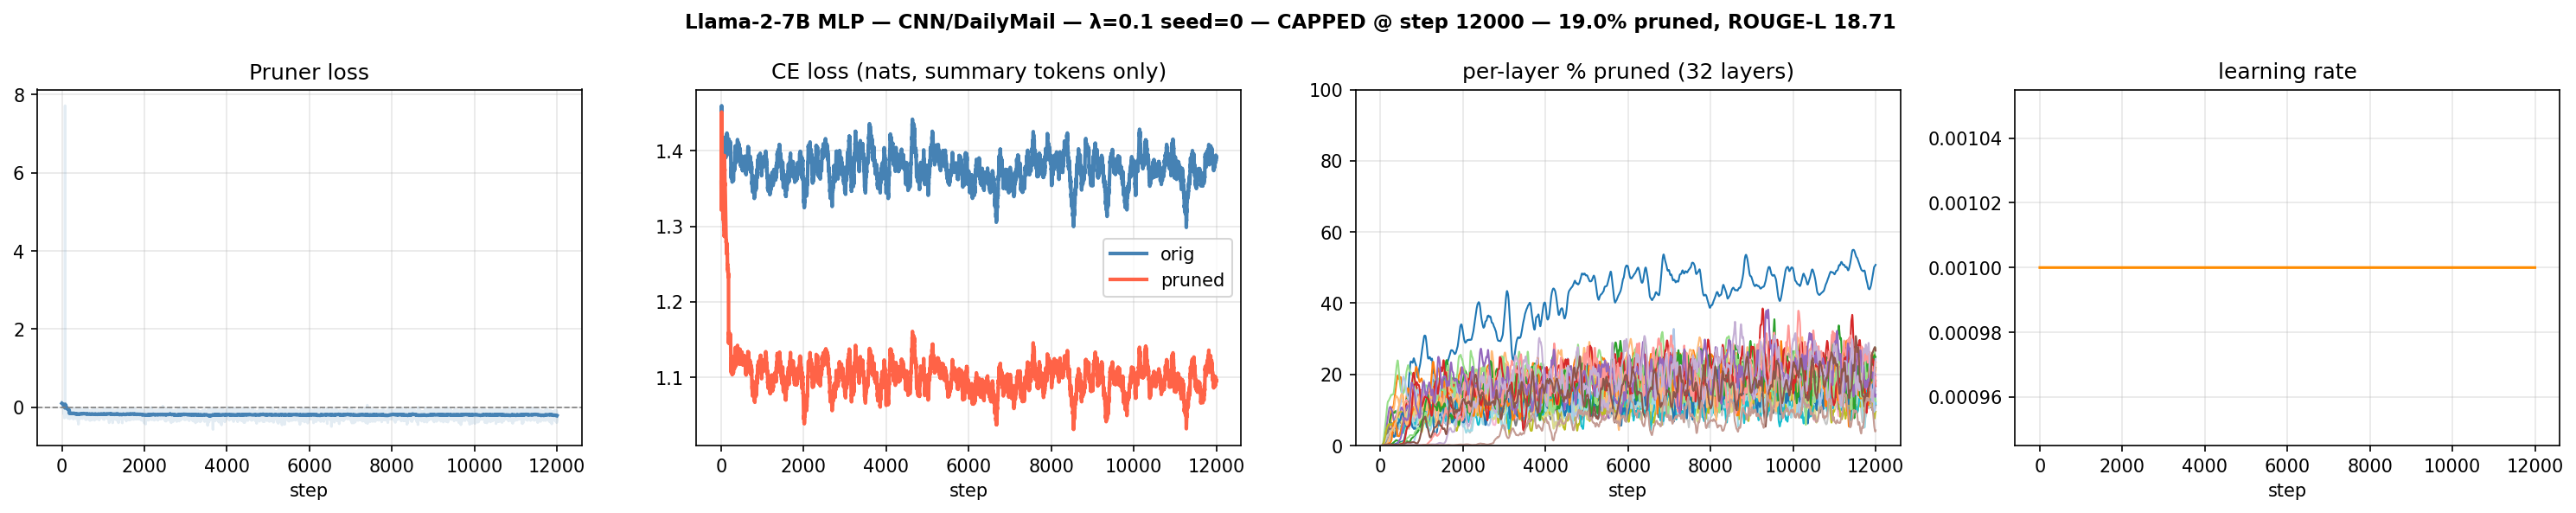
\includegraphics[width=\linewidth]{cnndm_lambda01.png}
    \column{0.5\textwidth}
      Target-only CE-delta objective (article masked from the loss, CE on the gold summary only) --- same training mechanism as WikiText-2, ported to a real downstream task.
      \vspace{0.4em}

      $\lambda{=}0.1$, single seed, \textbf{capped} at 12{,}000 steps (never converged).
      \begin{itemize}
        \item test ppl: 3.750 $\to$ 2.881
        \item ROUGE-L: 13.31 $\to$ 18.71
      \end{itemize}
  \end{columns}
  \vspace{0.3em}
  \tk{Pruned beats dense on every metric --- flagged, not claimed: single non-converged run, no dense-fine-tune control yet, dense baseline itself may just be weak (non-instruction-tuned model, bare completion prompt).}
\end{frame}

% ============================================================
\section{Summary}
% ============================================================

\begin{frame}{Summary}
  \begin{itemize}
    \item Same pruner, zero architecture changes, ported to 7B scale across two model families and three datasets.
    \item \textbf{Convergence is now a checked fact}, not an assumed step count --- and the one point that fails the check is diagnosed mechanistically (LR/$\lambda$ coupling), not swept under the rug.
    \item \textbf{Beats DISP-LLM's own published numbers at every converged Llama-2-7B/WikiText-2 operating point.}
    \item \textbf{Downstream zero-shot accuracy tells a different story}: near-parity at light pruning, a real and growing deficit at heavy pruning --- reported honestly alongside the ppl win, not instead of it.
    \item First downstream-task pruning run (CNN/DailyMail) shows a striking single-run result --- explicitly a case study in progress, gated on a dense-fine-tune control before it means anything.
  \end{itemize}
\end{frame}

\begin{frame}[standout]
  Thank you.\\[0.6em]
  {\normalsize\normalfont Findings: \texttt{diary/crisp-findings.md} \;|\; Paper direction: \texttt{diary/final-paper-direction.md}}
\end{frame}

\end{document}
